\section{Gas, liner and casing temperatures through exhaustion}\label{sec:temperatures}
The gas boundary stays at 2504~K (2231~$^\circ$C). The exposed solid heats to
about 1076--1077~$^\circ$C at its highest saved hot-face sample. Convection
supplies heat across the difference between gas and wall temperatures,
while conduction, decomposition, gas release and char consumption carry
energy away from the surface. The casing heats later as the liner thins.
\begin{figure}[H]\centering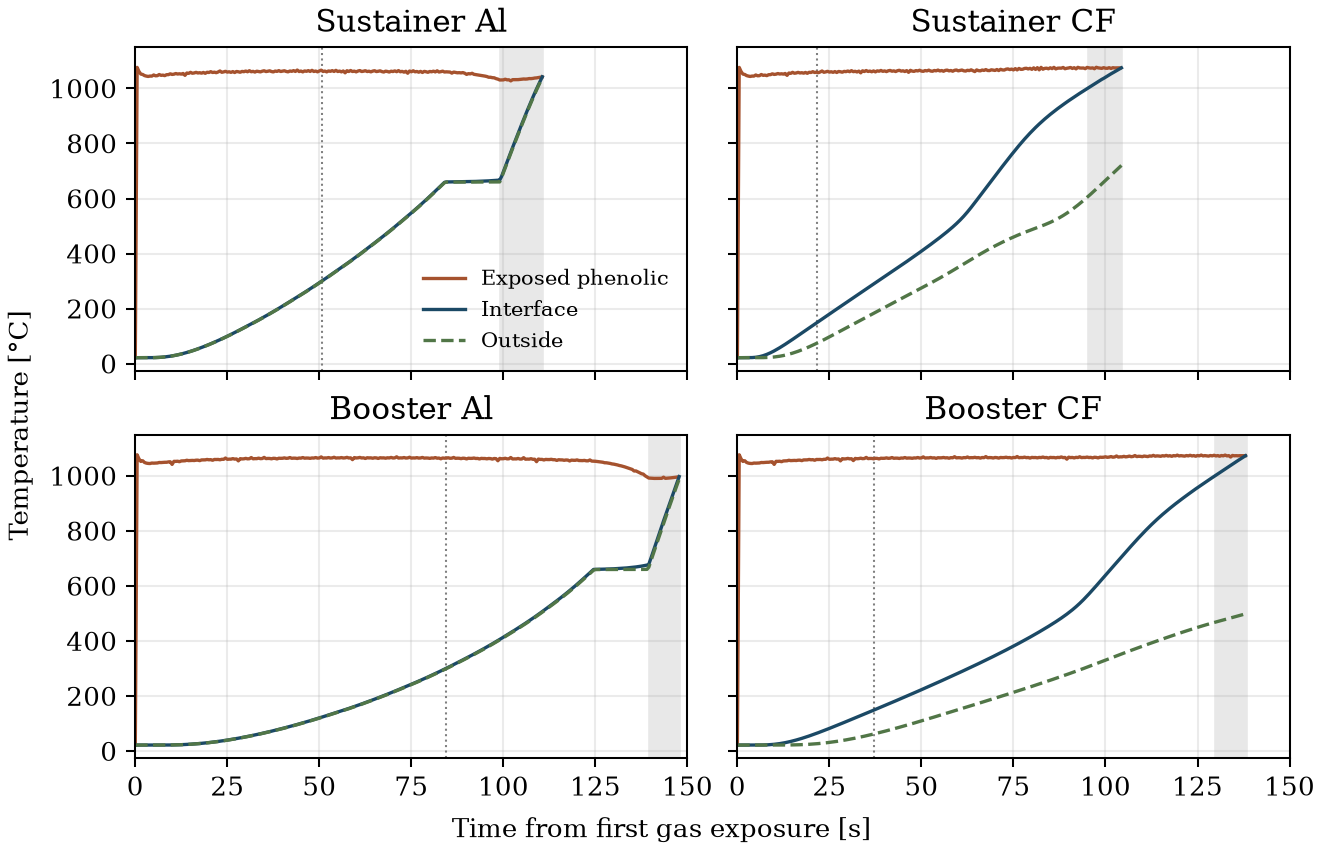
\includegraphics[width=.98\textwidth]{../analysis/whole_wall_temperatures.png}
\caption{Native ANSYS temperatures from first exposure. The dotted vertical line
marks the baseline casing-property flag (300~$^\circ$C Al, 150~$^\circ$C CF).
Shading begins when all Al is liquid or CF reaches 1000~$^\circ$C. The last
exposed-phenolic sample precedes exhaustion.}
\end{figure}
\begin{center}\small\begin{tabular}{lrrrrr}\toprule
& Baseline & Liquid Al or & Peak interface & Peak outside & Time of both\\
Motor & flag [s] & CF ceiling [s] & [$^\circ$C] & [$^\circ$C] & peaks [s]\\\midrule
Sustainer Al & 50.66 & 99.14 & 1042 & 1039 & 110.58 \\
Sustainer CF & 21.70 & 95.16 & 1075 & 720 & 104.33 \\
Booster Al & 84.36 & 139.44 & 997 & 988 & 147.75 \\
Booster CF & 37.24 & 129.78 & 1073 & 499 & 138.04 \\
\bottomrule\end{tabular}\end{center}
Both maxima use saved samples through liner exhaustion. The model ends there.
The CF casing sustains a larger inside-to-outside temperature difference than
the conductive Al surrogate. The assumed through-thickness CF properties and
retained backing geometry govern that result.
\clearpage
\section{Where pyrolysis occurs in the surviving liner}
The independent finite-volume model tracks virgin mass $m_v$ and char mass
$m_c$ in each surviving cell. With char yield $Y_c=600/1250=0.48$ the
converted fraction is $\alpha=m_c/(m_c+Y_c m_v)$. Thus a fully converted cell
can retain solid char. Geometric burnthrough requires that char to leave as well.
\begin{figure}[H]\centering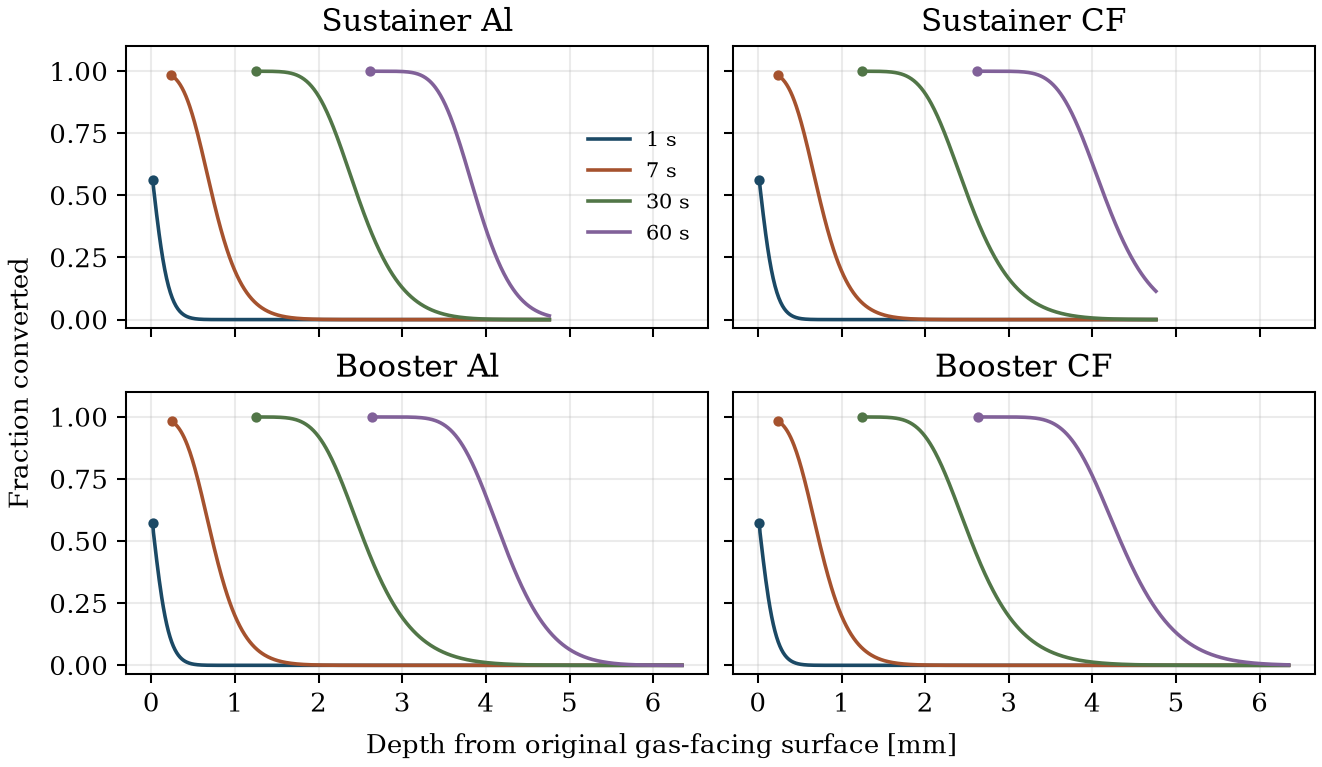
\includegraphics[width=.98\textwidth]{../analysis/whole_liner_conversion.png}
\caption{Nominal 640-cell liner profiles with evolving casings. Symbols locate
the first surviving cell centre. The interval to its left grows as material
leaves the wall. Depth is measured from the original inner wall.}
\end{figure}
\paragraph{Independent check of the native calculation.}
On the same 80/20-cell mesh and 40~ms maximum step the independent nodal
reduction reproduced each end of the native final interval within $10^{-8}$~s.
The nodal and native intervals overlap in all four cases. A separately
discretized finite-volume wall gives the following results.
\begin{center}\small\begin{tabular}{lrrr}\toprule
Motor & Native last step [s] & Reference FV last step [s] & Gap [ms]\\\midrule
Sustainer Al & 110.5398--110.5760 & 110.4600--110.4736 & 66.2 \\
Sustainer CF & 104.2956--104.3316 & 104.2400--104.2537 & 42.0 \\
Booster Al & 147.7099--147.7456 & 147.6000--147.6097 & 100.2 \\
Booster CF & 138.0053--138.0412 & 137.9400--137.9464 & 58.8 \\
\bottomrule\end{tabular}\end{center}
These raw integration intervals identify the last positive thickness and
the first zero thickness in each computation. The separation quantifies the
remaining difference between methods. The refinement comparisons on
pages~\pageref{sec:intervals}--\pageref{sec:matched} support the rounded
exposure times on the first page.
\clearpage
